\section{Processed Data}

\subsection{Velocity}

	\subsubsection{Sample Calculations}
	
	\begin{align*}
		\bar{v} &= \frac{\text{distance traveled by water}}{\text{time taken}} \\
		\bar{v}_{\text{Site 1}} &= 0.5725 \text{ m/s} \\
		\bar{v}_{\text{Site 2}} &= 0.24 \text{ m/s} \\
		&\vdots \\
		\bar{v}_{\text{Site 8}} &= 0.03334 \text{ m/s}
	\end{align*}
	
	\subsubsection{Results}
	
	\begin{figure}[H]
		\centering
		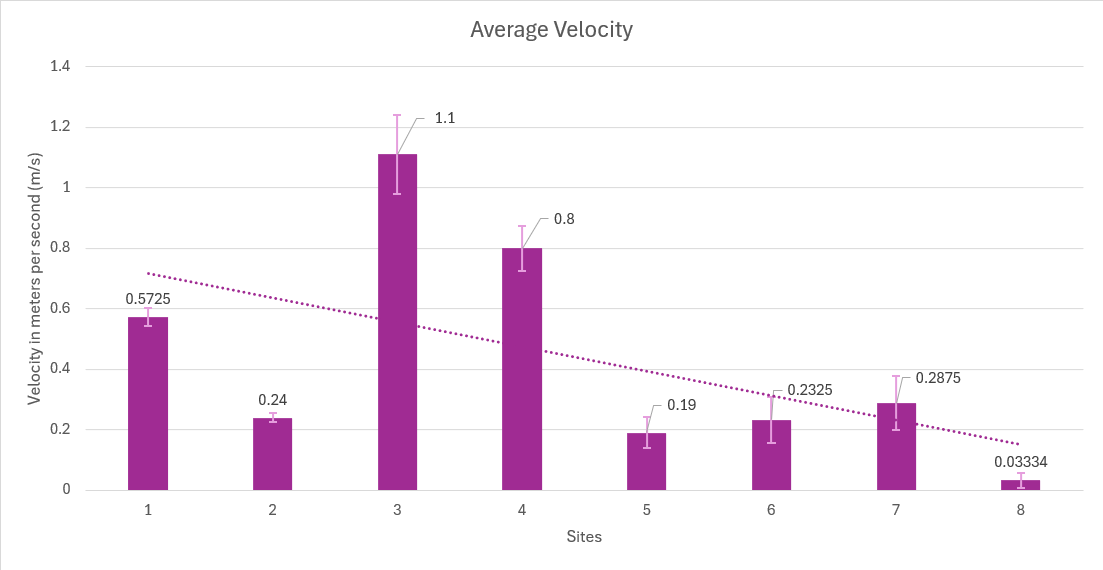
\includegraphics[width=1.0\textwidth]{Images/AverageVelocity.png}
		\caption{Average Velocity at Each Site}
	\end{figure}
	

\subsection{Channel Width}

	\subsubsection{Sample Calculations}
	
	\begin{align*}
		\text{Width} &= \text{measured distance across the water surface at each site} \\
		W_{\text{Site 1}} &= 2.02 \text{ m} \\
		W_{\text{Site 2}} &= 4.19 \text{ m} \\
		&\vdots \\
		W_{\text{Site 8}} &= 4.24 \text{ m}
	\end{align*}

	\subsubsection{Results}

\begin{figure}[H]
	\centering
	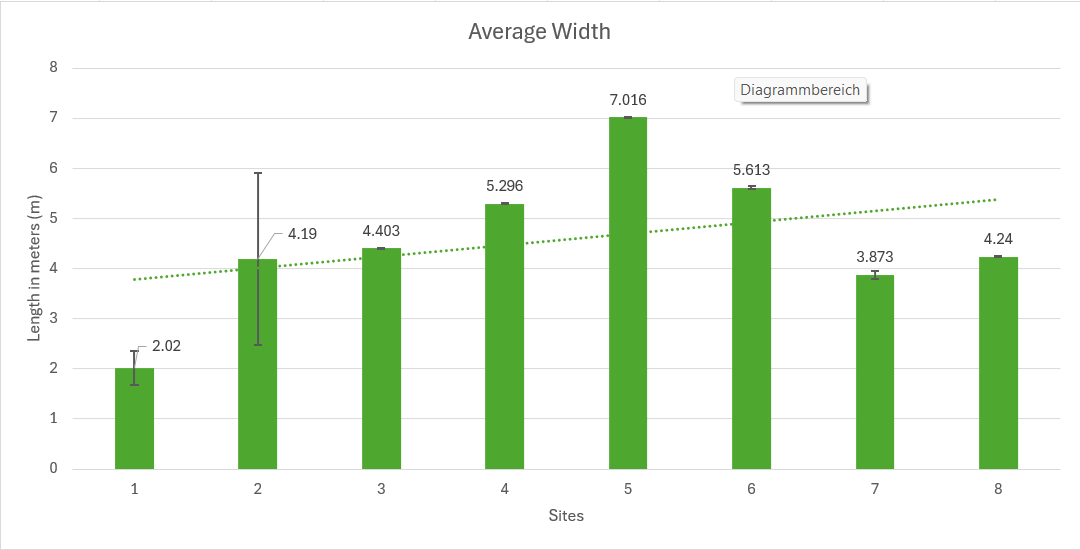
\includegraphics[width=1.0\textwidth]{Images/AverageWidth.png}
	\caption{Average Channel Width at Each Site}
\end{figure}


\subsection{Channel Depth}

	\subsubsection{Sample Calculations}
	
	\subsubsection{Sample Calculations}
	\begin{align*}
		\text{Depth} &= \frac{\text{sum of measured depths at intervals}}{\text{number of measurements}} \\
		D_{\text{Site 1}} &= 0.145 \text{ m} \\
		D_{\text{Site 2}} &= 0.179 \text{ m} \\
		&\vdots \\
		D_{\text{Site 8}} &= 0.280 \text{ m}
	\end{align*}
	
	\subsubsection{Results}

\begin{figure}[H]
	\centering
	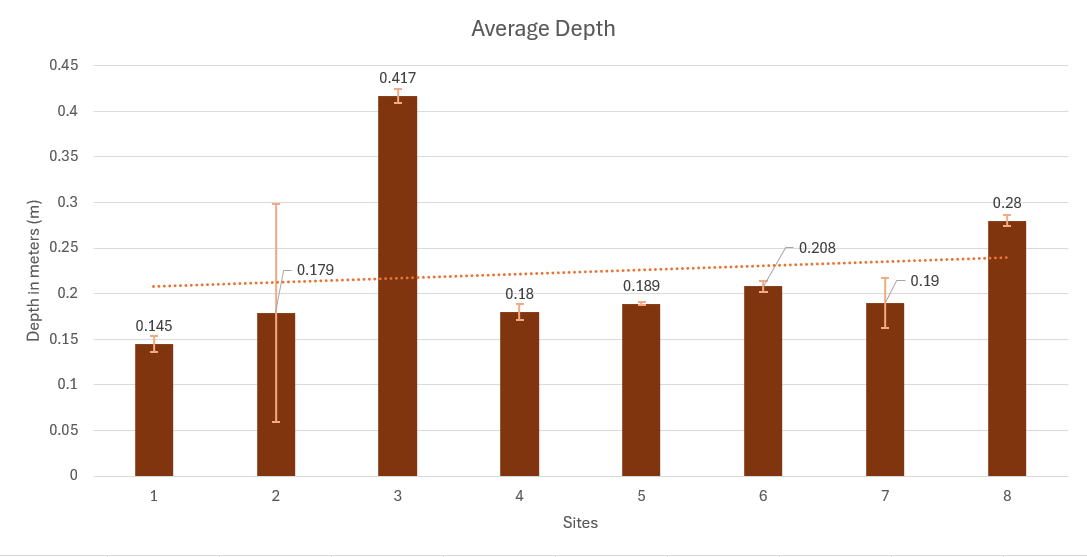
\includegraphics[width=1.0\textwidth]{Images/AverageDepth.png}
	\caption{Average Channel Depth at Each Site}
\end{figure}


\subsection{Wetted Perimeter}

	\subsubsection{Sample Calculations}
	
	\begin{align*}
		P &= \text{sum of the lengths of all wetted edges of the channel} \\
		P_{\text{Site 1}} &= 2.03 \text{ m} \\
		P_{\text{Site 2}} &= 2.96 \text{ m} \\
		&\vdots \\
		P_{\text{Site 8}} &= 4.67 \text{ m}
	\end{align*}
	

	\subsubsection{Results}
	
	% Wetted Perimeter
	\begin{figure}[H]
		\centering
		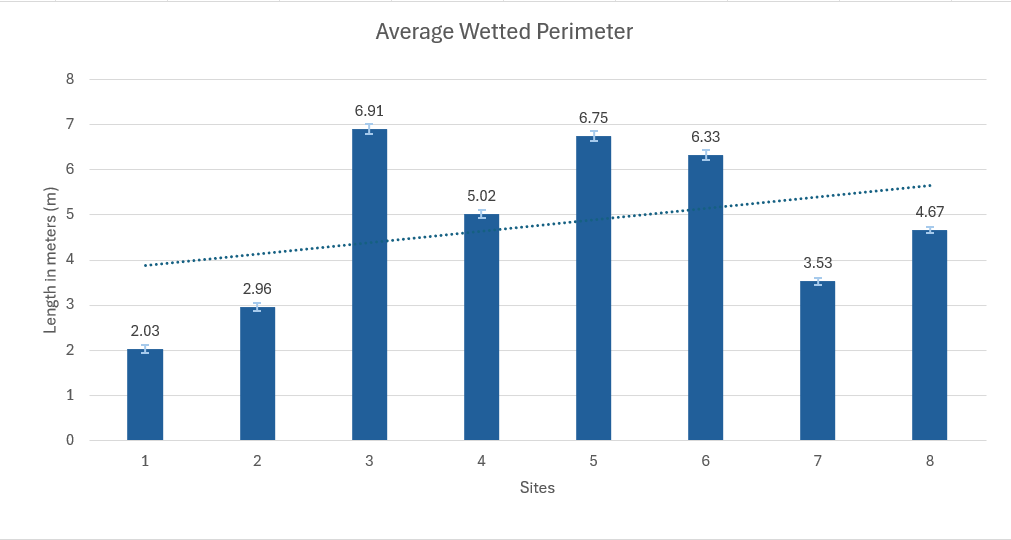
\includegraphics[width=1.0\textwidth]{Images/AverageWettedPerimeter.png}
		\caption{Wetted Perimeter at Different Sites}
	\end{figure}
	
\subsection{Cross-Sectional Area}

	\subsubsection{Sample Calculations}
	
	\begin{align*}
		A &= \text{Mean Width} \times \text{Mean Depth} \\
		A_{\text{Site 1}} &= 2.02 \times 0.145 = 0.2929 \text{ m$^2$} \\
		A_{\text{Site 2}} &= 4.19 \times 0.179 = 0.75001 \text{ m$^2$} \\
		&\vdots \\
		A_{\text{Site 8}} &= 4.24 \times 0.28 = 1.1872 \text{ m$^2$}
	\end{align*}
	

	\subsubsection{Results}
	
	\begin{figure}[H]
	\centering
	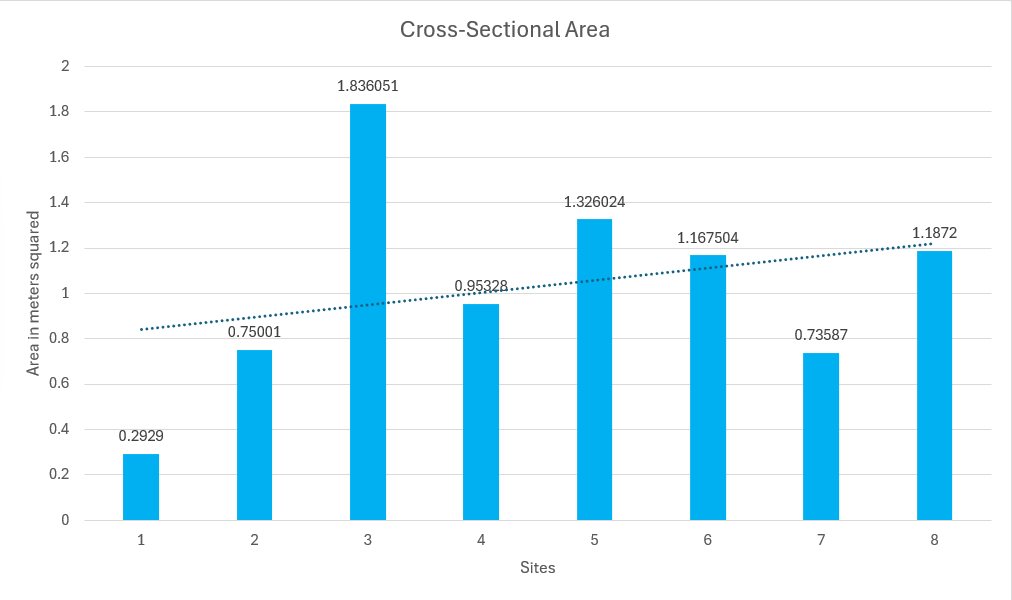
\includegraphics[width=1.0\textwidth]{Images/Cross-SectionalArea.png}
	\caption{Cross-Sectional Area at Different Sites}
\end{figure}

\subsection{Channel Efficiency}

	\subsubsection{Sample Calculations}
	
	%\includegraphics[width=0.7\textwidth]{Images/xx.jpg}\par\vspace{1.5cm}
	
	\begin{enumerate}
		\item Channel efficiency = Hydraulic radius -> The higher the radius, the greater the efficiency.
		\item $\text{Cross-Sectional Area}\div\text{Wetted Perimeter} = \text{Hydraulic Radius}$
	\end{enumerate}
	
	
	\begin{align*}
		R &= \frac{A}{P} \\
		R_{\text{Site 1}} &= \frac{4.08}{2.03} = 2.01 \text{ m} \\
		R_{\text{Site 2}} &= \frac{17.56}{2.96} = 5.932 \text{ m} \\
		&\vdots \\
		R_{\text{Site 8}} &= \frac{17.98}{4.67} = 3.85 \text{ m}
	\end{align*}
	
		\subsubsection{Results}
		
		\begin{table}[H]
			\centering
			\begin{tabularx}{\textwidth}{l *{3}{Y}}
				\hline
				Sites & Wetted Perimeter $P$ (m) & Cross-sectional Area $A$ (m$^2$) & Channel Efficiency $R=A/P$ (m) \\
				\hline
				Site 1 & 2.03 & 4.08  & 2.01 \\
				Site 2 & 2.96 & 17.56 & 5.932 \\
				Site 3 & 6.91 & 19.39 & 2.806 \\
				Site 4 & 5.02 & 28.05 & 5.588 \\
				Site 5 & 6.75 & 49.22 & 7.292 \\
				Site 6 & 6.33 & 31.51 & 4.978 \\
				Site 7 & 3.53 & 15.00 & 4.249 \\
				Site 8 & 4.67 & 17.98 & 3.85 \\
				\hline
			\end{tabularx}
			\caption{}
			\label{tab:channel_efficiency}
		\end{table}

% Channel Efficiency
\begin{figure}[H]
	\centering
	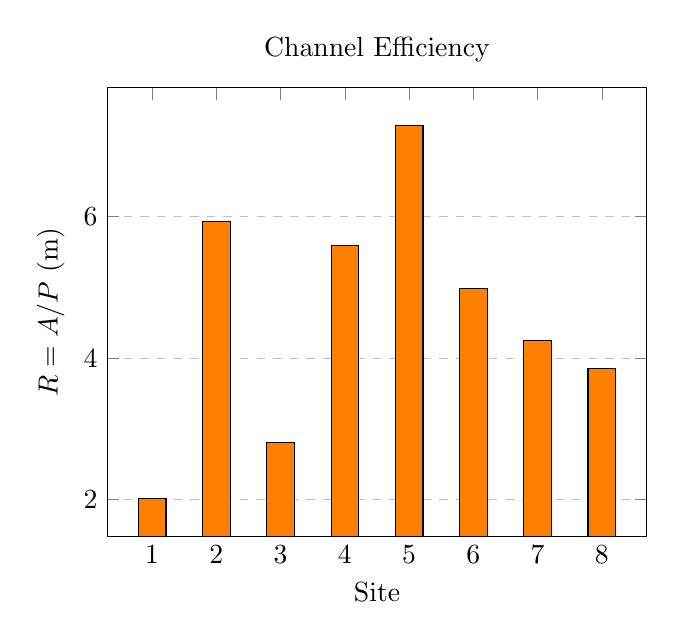
\begin{tikzpicture}
		\begin{axis}[
			title={Channel Efficiency},
			xlabel={Site},
			ylabel={$R=A/P$ (m)},
			xtick=data,
			xticklabels={1,2,3,4,5,6,7,8},
			ymajorgrids=true,
			grid style=dashed
			]
			\addplot[ybar,fill=orange] coordinates {
				(1,2.01) (2,5.932) (3,2.806) (4,5.588) (5,7.292) (6,4.978) (7,4.249) (8,3.85)
			};
		\end{axis}
	\end{tikzpicture}
	\caption{Channel Efficiency at Different Sites}
\end{figure}

\subsection{Discharge}
	
	\subsubsection{Sample Calculations}
	
	\subsection{River Discharge}
	
	\begin{enumerate}
		\item $\text{Discharge (cumecs)}= \text{Cross-Sectional Area}\ (\si{\metre\squared}) \times \text{Velocity}\ (\si{\metre\per\second})$
		\item Use mean depth and mean width to measure cross-sectional area (\si{\metre\squared}).
		\item Measure velocity either through digital flow-meter or with a stopwatch, a cork,measuring tape and ranging poles ($\times 4$)
		\item Then use the average velocity and multiply it by the area to get the discharge
	\end{enumerate}
	
	\begin{align*}
		Q &= A \times \bar{v} \\
		Q_{\text{Site 1}} &= 4.08 \times 0.5725 = 2.34 \text{ m$^3$/s} \\
		Q_{\text{Site 2}} &= 17.56 \times 0.24 = 4.21 \text{ m$^3$/s} \\
		&\vdots \\
		Q_{\text{Site 8}} &= 17.98 \times 0.03334 = 0.60 \text{ m$^3$/s}
	\end{align*}
	
		\subsubsection{Results}
		
		\begin{table}[H]
			\centering
			\begin{tabularx}{\textwidth}{l *{3}{Y}}
				\hline
				Sites & Cross-sectional Area $A$ (m$^2$) & Velocity $\bar{v}$ (m/s) & Discharge $Q=A \times \bar{v}$ (m$^3$/s) \\
				\hline
				Site 1 & 4.08  & 0.5725  & 2.34 \\
				Site 2 & 17.56 & 0.24    & 4.21 \\
				Site 3 & 19.39 & 1.110   & 21.51 \\
				Site 4 & 28.05 & 0.80    & 22.44 \\
				Site 5 & 49.22 & 0.19    & 9.35 \\
				Site 6 & 31.51 & 0.2325  & 7.33 \\
				Site 7 & 15.00 & 0.2875  & 4.31 \\
				Site 8 & 17.98 & 0.03334 & 0.60 \\
				\hline
			\end{tabularx}
			\caption{}
			\label{tab:discharge}
		\end{table}

% Discharge
\begin{figure}[H]
	\centering
	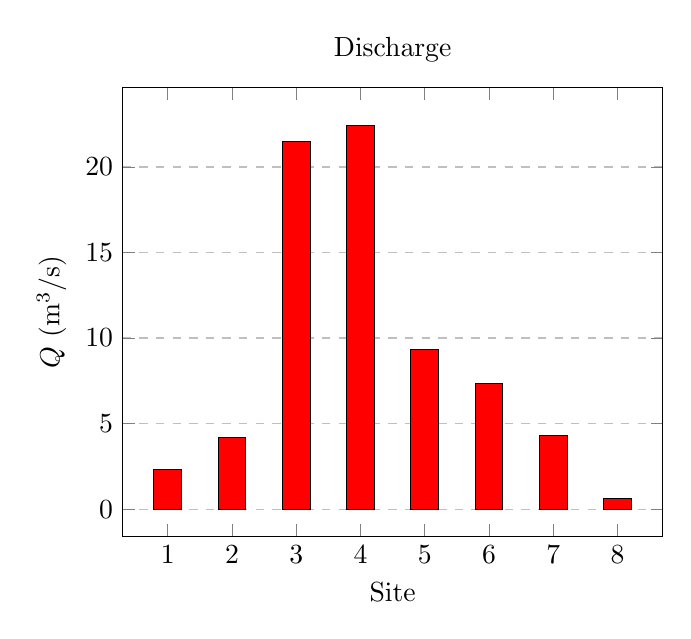
\begin{tikzpicture}
		\begin{axis}[
			title={Discharge},
			xlabel={Site},
			ylabel={$Q$ (m$^3$/s)},
			xtick=data,
			xticklabels={1,2,3,4,5,6,7,8},
			ymajorgrids=true,
			grid style=dashed
			]
			\addplot[ybar,fill=red] coordinates {
				(1,2.34) (2,4.21) (3,21.51) (4,22.44) (5,9.35) (6,7.33) (7,4.31) (8,0.60)
			};
		\end{axis}
	\end{tikzpicture}
	\caption{Discharge at Different Sites}
\end{figure}

\subsection{Bedload Size}

	\subsubsection{Sample Calculations}
	
	\begin{align*}
		\text{Average Bedload Size} &= \frac{\text{Sum of measured sizes}}{\text{Number of particles}} \\
		\text{Site 1} &= 90.20 \text{ mm} \\
		\text{Site 2} &= 84.40 \text{ mm} \\
		&\vdots \\
		\text{Site 8} &= 17.60 \text{ mm}
	\end{align*}
	
		\subsubsection{Results}
		
% Bedload Size
	\begin{figure}[H]
		\centering
		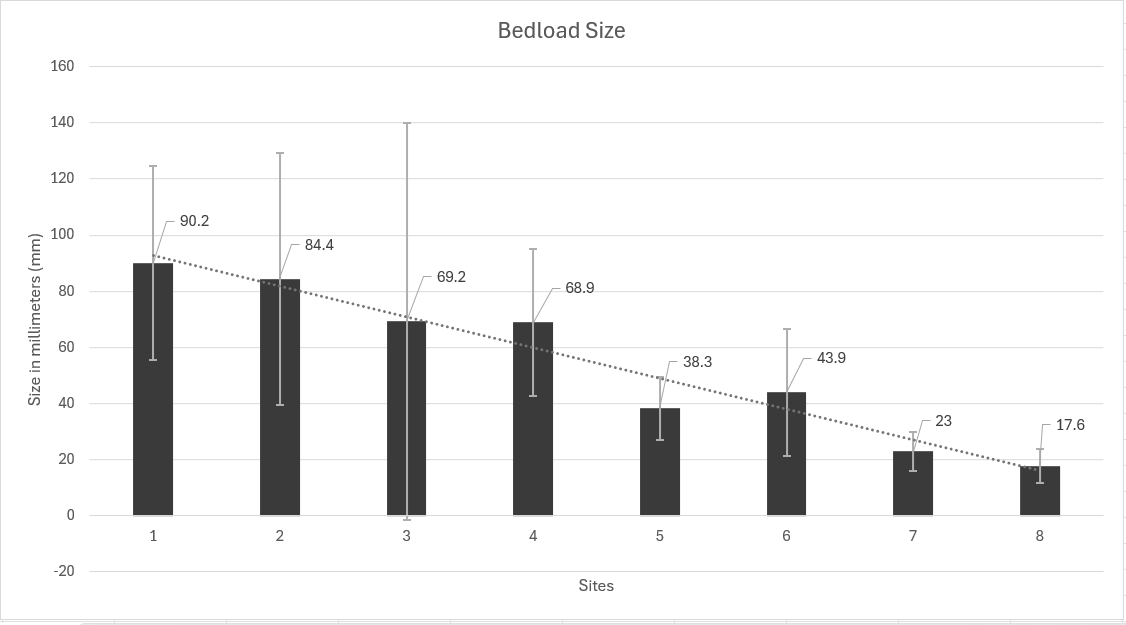
\includegraphics[width=1.0\textwidth]{Images/AverageBedloadSize.png}
		\caption{Bedload Size at Different Sites}
		\end{figure}
		


